% ----------------------------------------------------------------
% Article Class (This is a LaTeX2e document)  ********************
% ----------------------------------------------------------------
\documentclass[12pt]{article}
\usepackage[english]{babel}
\usepackage{amsmath,amsthm}
\usepackage{graphicx}
\usepackage{caption}
\usepackage{listings}
\usepackage{color}
\usepackage{subcaption}
\usepackage{amsfonts}
\usepackage{float}
\usepackage{indentfirst}
\usepackage{lscape}
\usepackage[top=2.5cm,bottom=2.5cm,right=2.5cm,left=2.5cm]{geometry}
\usepackage{titlesec}
\setcounter{secnumdepth}{5}


% THEOREMS -------------------------------------------------------
\newtheorem{thm}{Theorem}[section]
\newtheorem{cor}[thm]{Corollary}
\newtheorem{lem}[thm]{Lemma}
\newtheorem{prop}[thm]{Proposition}
\theoremstyle{definition}
\newtheorem{defn}[thm]{Definition}
\theoremstyle{remark}
\newtheorem{rem}[thm]{Remark}
\numberwithin{equation}{section}
% ----------------------------------------------------------------
\begin{document}
\title{Project of first year master degree}%
\author{Etienne Caillaud, Thomas Le Bris, Ibrahima Gueye, Gaetan Adier}%
\maketitle
\newpage

\tableofcontents
\newpage
% ----------------------------------------------------------------

\section{Introduction}

\section{Team presentation}

\section{User requirement}

\newpage
\section{State of art}

Color image processing has become a major issue since a few years, most of the colour texture discrimination having been explored using the marginal colours way. The issue is that we are now able to do colour image recognition on digital images but the results on nature pictures are rather mediocre.

The CLEF contest has been created as an answer to that problematic, making universities' and laboratories' own solutions compete against each other in order to find the best colour texture feature.

In this document we will introduce key-points and their use in the various descriptors. We will go first with the standard ones which are SIFT SURF and opponent SIFT. The last one being the descriptor used by FINKI, the laboratory from the last year contest we chose as reference to compare our results. We will then use a new descriptor offered by Noel Richard, the C$_2$O.


\subsection{Key-points}

\subsubsection{Scale-space extrema detection}

For this type of key-point detection, the aim is to only retrieve the useful key-points (which are characterizing the image the best) without taking an "abstract" of the whole image as the dense grid method.
To do it, the first thing that is done is to create a pyramidal tree containing some copies of the image at different resolutions. These copies will be blurred by different Gaussian filters.
\begin{equation}
L(x,y,k\sigma)=G(x,y,k\sigma)*I(x,y)
\end{equation}

The images are grouped by octaves (an octave being a level of the pyramidal tree). The resolution is divided by 2 with each consecutive octave : for the difference of Gaussians, it's equivalent to multiply $\sigma$ by 2.
\begin{equation}
D(x,y,\sigma)=L(x,y,k_i\sigma)-L(x,y,k_j\sigma)
\end{equation}

%For each octave, it's made a difference between each two consecutive images blur by the filter at scale $k*\sigma$.
Then, for each octave, the difference between every two consecutive blurred images (by the filter at scale $k*\sigma$) is computed.
%This difference result is that the objects that are remaining on the difference image are thus which size is included between $\sigma$ and $k*\sigma$.The parameter k is a constant of the algorithm that is fixed following a precise rule which depend on the precision that the user would.
The remaining objects on the image obtained are the ones which size is included between $\sigma$ and $k*\sigma$. The parameter k is a constant defined according to the precision wanted.

Thanks to the different resolutions, for each octave the difference result will keep higher and higher object that will allow us to detect approximately all the sizes of important features on the image.
With all these difference calculated, the algorithm will take the maxima of each one as key-points.

\begin{figure}[h]
    \center
    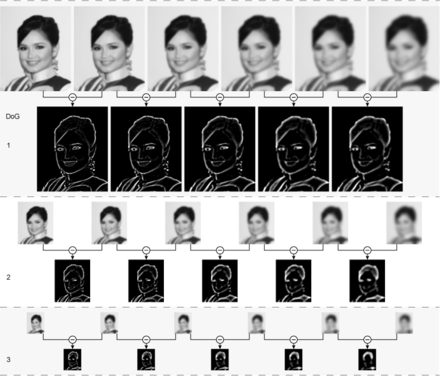
\includegraphics[scale=0.6]{DoG.png}
    \caption{Difference of Gaussians illustration (example from wikipedia)}\label{fig:Difference of Gaussians}
\end{figure}
After doing that, the algorithm must discriminate and precise the coordinate of a part of the key-point. Indeed, using different resolutions give some imprecise coordinate so it's necessary to make an interpolation to obtain the coordinate corresponding to the original image for key-point extracted from the most reduced resolutions images.  It is necessary to remove some kind of point too. The points that have not enough contrast comparing to the other are removed as the points that are on ridges (these points are really unstable and could move or disappear for many reasons so it's better to remove them).

When these operations have been computed, we obtain a set of key-points that characterize the image. This method allows to obtain the key-points to characterize an image without taking a predefined set of point. So the set of points obtained is potentially lighter than the one obtained by the dense grid method and it is more accurate because only important points wherever they are are conserved.


\subsubsection{Dense Grid}
The dense grid method is the easiest way to extract key-points.
The image has first to be divided into k sub-images and the intersections of the sub-images' outlines become the key-points.

\begin{figure}[h]
    \center
    \includegraphics[scale=0.7]{Dense_grid.png}
    \caption{Dense grid}\label{fig:dense_grid}
\end{figure}

\subsection{Descriptors}
The detection of key-points in images is increasingly used because it helps to do many tasks for example recognition, images assembly, 3D modeling, image indexation, video tracking etc. The key-points extraction in one image allows characterizing this image. Comparing the key-points of two images we can deduce if they have common information or not.
\subsubsection{SIFT}
SIFT (scale-invariant feature transform) is an algorithm used in sector of computer vision for detection and identification of similar elements between different numeric images.
The principal method proposed by the author David Lowe is to calculate the SIFT descriptors on images studied. These descriptors are numeric information which derived of local analysis of the image and they characterize the visual content of this image so that this one is independent of the scale, the framing, the angle of observation and the luminosity.
\begin{itemize}
	
	\item Orientation assignment: On the base of local image gradient detections each key-point detected is assigned to one or many orientations. Insofar as descriptors are calculated from these orientations, it is important to safeguard the invariance of these descriptors to the rotation because whatever the orientation we must obtain the same descriptors using the same image.

For example with a key-point ($x_0$,$y_0$,$\sigma_0$), the calculation is done on the Gradient of the pyramid L(x,y,$\sigma_0$) which factor is nearest the scale factor of the point. In this way the calculation is also independent to the scale variance. With the symmetric finite difference, the gradient and the amplitude are calculated for each position around the key-point.
The calculation of these two factors is given by the following relations:
$$m(x,y)=\sqrt{(L(x+1,y)-L(x-1,y))^2+(L(x,y+1)-L(x,y-1))^2}$$
$$\theta(x,y)=atan2(L(x,y+1)-L(x,y-1),L(x+1,y)-L(x-1,y))$$
A histogram with 36 intervals is realized on the vicinity and each interval covering an angle of 10 degrees.

\begin{figure}[h]
    \center
    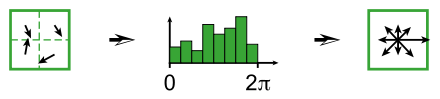
\includegraphics[scale=1]{SIFT_histogram_construction.png}
    \caption{SIFT histogram construction}\label{fig:SIFT_histogram_construction}
\end{figure}

On one hand, the histogram is moderated by a Gaussian window circular with a factor equal to 1.5 times of the scale factor of the key-point . On the other hand by the amplitude of each point. The peaks in this histogram correspond to the dominant orientations. All dominant orientations allow to have at least 80\% of the maximum value are taking in consideration and other additional key-points are detected. These new key-points detected are only different by the principal orientation.

	\item key-point descriptor: In this stage, a descriptor vector is created for each key-point detected such the descriptor is distinctive and invariant to the remaining variations like illumination, 3D viewing, etc. This stage is made on image which is more near the scale of the key-point scale.

The local system coordinates is modified for guarantee the invariance to the rotation by using an angle rotation equal to the orientation of the key-point in reverse direction.  Then, an area of 16x16 pixels is taken around the key-point; subdivide in 4x4 zones of 4x4 pixels each one. A histogram including 8 intervals is calculated on each zone. At each point of the zone, the orientation and the amplitude are calculated like previously. The orientation determines the interval to increment in the histogram which done by double weighted by the amplitude and by a center window Gaussian on the key-point of parameter 1.5 times of the scale factor of the key-point.

After that, the 16 histograms with 8 intervals each one, are concatenated and normalized. In object to reduce the sensibility of the descriptor to the changes of the luminosity, the values are fixed to 0.2 and the histogram is calculated again for finally give the descriptor of the key-point of 128 dimension.
\begin{figure}[h]
    \center
    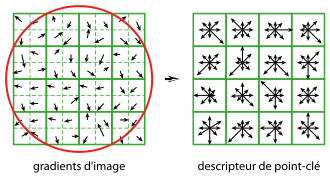
\includegraphics[scale=0.75]{SIFT_gradient_magnitude_and_orientation_computation.png}
    \caption{SIFT gradient magnitude and orientation computation}\label{fig:SIFT_gradient_magnitude_and_orientation_computation}
\end{figure}


\end{itemize}


\subsubsection{SURF}

SURF for Speeded Up Robust Features is an descriptor and algorithm of feature detection. It also used in the sector of computer vision and image understanding for objects detection or 3D reconstruction.

SURF is in part inspired by the SIFT descriptor but it is more fast from a time calculation point of view. According to the authors, it is also more robust for different image transformations.

SURF is based on sums of Haar 2D wavelets responses and uses efficiently the integrals images.
	
		

\subsubsection{Opponent SIFT}

The opponent SIFT descriptor is an algorithm using the same method as the standard SIFT descriptor except for the fact that it calculates three descriptors for each Key-points, obtained from the color opponent channel and defined as

\begin{equation}
O_{1} = \frac{R - G}{\sqrt{2}}, O_{2} = \frac{R + G - 2B}{\sqrt{6}}, O_{3} = \frac{R + G + B}{\sqrt{3}}.
\end{equation}

The opponent SIFT describes the three opponent color spaces : the two first channels $O_1$, $O_2$ contain some intensity information, but they are sensible to changes in light intensity. The last channel will contain the intensity information.

The strength of this method is that it uses a color space, and we can see directly information of that with the algorithm of the SIFT descriptor. The weakness is that the color space used is the RGB one.

\subsubsection{C$_2$O}

C$_2$O feature is a color descriptor which aim is to characterize an image by its color and texture characteristics. Indeed, the descriptors previously presented are satisfying to characterize images in gray or color levels but are pretty weak for highly textured images like nature pictures.
That's why the university of Poitiers has worked on a descriptor named C$_2$O (Color Contrast Occurrence), based on a vector including texture and color information.
To compute it, there is two steps to follow : the calculation of the Color Contrast Occurrence Matrix and the extraction of the feature (descriptor) from the matrix.



\paragraph{The Color Contrast Occurrence Matrix}
~~\\
~~\\
To compute this descriptor, the aim is to calculate a matrix which represents each key-point by a probability.
To compute it, the image has to be used in a color space which is able to separate best the color and the luminance information. Tests have shown that the CIE L* a* b* space separate "has minimum correlation between luminance and chrominance information" ("Color Contrast Occurrence, a full vector for color and texture").
So the image is passed in the CIE L* a* b* color space before the calculation of the descriptor.
Before the calculation of the L* a* b* space, its needed to transform our image through the XYZ space that is a perceptual space based on a linear transformation of the RGB space.


\vspace{0.5cm}
$$A=\begin{pmatrix}
	X_r&X_g&X_b\\
	Y_r&Y_g&Y_b\\
    Z_r&Z_g&Z_b
\end{pmatrix}$$
\vspace{0.5cm}
\begin{equation}
\begin{pmatrix}X\\Y\\Z\end{pmatrix}=A*\begin{pmatrix}R\\G\\B\end{pmatrix}
\end{equation}

With A a matrix which coefficients are depending on the chosen standard illuminant.
When this XYZ space has been computed, we have to compute the following transformation to get our image in the L* a* b* space.

\vspace{0.5cm}
\begin{equation}
L^*=  \left \{
   \begin{array}{l}
      116*(\frac{Y}{Y_0})^\frac{1}{3}-16~~~~si \frac{Y}{Y_0}>0.008856\\
   903.3*(\frac{Y}{Y_0})~~~~~~~~~~si \frac{Y}{Y_0}<0.008856\\
   \end{array}
   \right .
\end{equation}
\vspace{0.5cm}
\begin{equation}
a^*=500*\begin{bmatrix}f(\frac{X}{X_0})-f(\frac{Y}{Y_0})\end{bmatrix}
\end{equation}
\vspace{0.5cm}
\begin{equation}
b^*=200*\begin{bmatrix}f(\frac{Y}{Y_0})-f(\frac{Z}{Z_0})\end{bmatrix}
\end{equation}
After that, we can calculate the descriptor. The principle is simple : for each key-point, we have to calculate the probability to have a specific color difference between two pixels separated by a spatial vector (a voir si le dit vecteur est vecteur type). The color difference is calculated by considering the angles created by the L* a* b* representation and a perceptual distance (probablement sur la luminance mais a v�rifier).


So we define the color contrast occurrence value as : $\overrightarrow{\Lambda(C_i,C_j)}$
\begin{equation}
\overrightarrow{\Lambda(C_i,C_j)} : prob(\overrightarrow{\Lambda(C_i,C_j)} = \overrightarrow{\Lambda_\chi}
\end{equation}
\begin{equation}
~~~~~~~~~~~~~~~~~~~~ with~ \|\overrightarrow{\Lambda(C_i,C_j)}\| = \Delta E_\chi
\end{equation}
\begin{equation}
~~~~~~~~~~~~~~~~~~~~~~~~~~ and ~ \,(\overrightarrow{Oa},\overrightarrow{c_ic_j}) = (\alpha,\beta) = \,\overrightarrow{\Lambda_\chi}
\end{equation}

This computation gives us a cloud of point which characterizes the key-point by its color and texture neighborhood (see below).

\begin{figure}[h]
    \center
    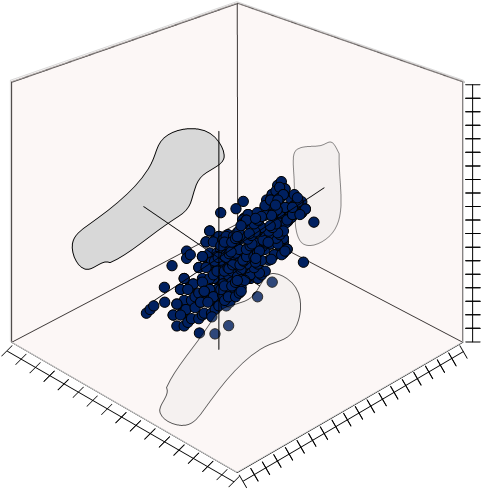
\includegraphics[scale=0.45]{IllustrationMatriceC2O.png}
    \caption{Color Contrast Occurrence Matrix}\label{fig:Color Contrast Occurence Matrix}
\end{figure}

On the figure shown above, we can see an example of the cloud of points that we expect to obtain. There are two thing which characterize the image :
\begin{itemize}
\item the size and the form of the cloud characterizing the texture around the key-point.
\item the projections on the three plans of the representation which characterize the density of the cloud of points.
\end{itemize}
\paragraph{The Color Contrast Occurrence feature}
~~\\
~~\\
With the cloud of point obtained by the computation of the Color Contrast Occurrence matrix, we have a 3 dimensional representation of our key-point. To reduce the quantity of data to store and to facilitate the distance calculation, we have to represent this matrix by at least a 2-dimensional feature.
To do that, the solution used is to realize a spherical quantization on the cloud of point to have a histogram which will represent our key-point on two dimensions.
Mathematically, this quantization is expressed as follows :

\begin{equation}
Sig_{C_2O}(I) = h_{\Delta i\alpha j\beta k)} = prob(\Delta_i\leq\|\overrightarrow{\Lambda(C_i,C_j)}\|<\Delta_j+\Delta E_{step})
\end{equation}

\begin{equation}
~~~~~~~~~~~~~~~ and~  \frac{2\pi}{n_{\alpha}}j \leq \alpha < \frac{2\pi}{n_{\alpha}}(j+1)
\end{equation}
\begin{equation}
~~~~~~ and~ 0 \leq \beta < \frac{2\pi}{n_{\beta}}(k)
\end{equation}

Each sphere will include a number of points of the cloud, but to have a better distribution, each sphere will be split in some part as shown below :

\begin{figure}[h]
    \center
    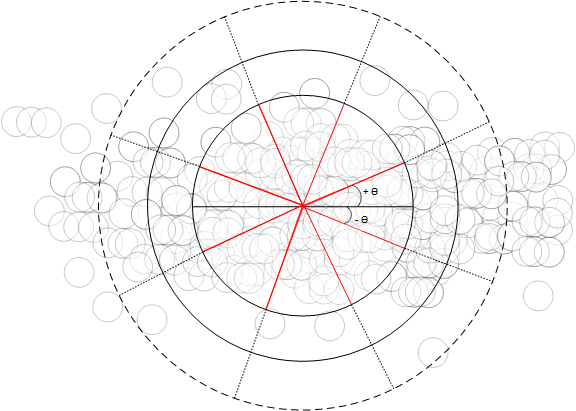
\includegraphics[scale=0.65]{QuantificationSpherique.png}
    \caption{Spheric quantizaton}\label{fig:Qantification sph�rique}
\end{figure}



Here we can see a sectional view of our spherical quantization. Each sphere is divided by n parts as shown above, and the number of points in each part are concatenated one by one in the description vector (quarter after quarter and sphere after sphere).
\newpage

\section{Work done}

\subsection{Process flow}

What we call process flow in this project is the main function of the project. Indeed in that function we have to manage almost all the others function, and more precisely features function, classification function, test and validation function, or create or manage the directory files.
This program is make that we can change the different descriptors (SIFT C$_2$O) as we want.
In this part we will present how works the sub-functions inside the process flow.

\subsubsection{Workspace}

The aim of the Process flow function is to allow at the user to choose his workspace, and choose where he want to write the results obtained by the software. Here we can see how the folder will be organize by using this function:

\begin{figure}[h]
    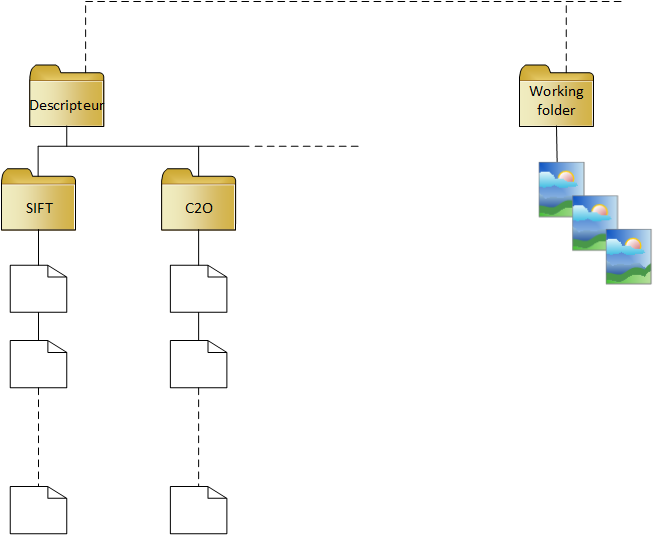
\includegraphics[scale=0.7]{arborescence.png}
    \caption{Organization of the workspace}\label{fig:process1}
\end{figure}

 Indeed we can see that we create a folder descriptor, if he is not create yet, in this folder we create as much folders as the user wants. For this he just has to enter the name he wants in the parameter \textit{name\_desc}. We can also see, the user can choose the work folder he wants.

\subsubsection{Processing}

The second goal of this function is to compile the whole processing, so if the user wants to compile one particular function in the software he should not use the function \textit{Process\_flow}. In this function we will found this line-up:

\begin{itemize}
\item Creation of folders and path to the workspace
\item Calculation of descriptors and link with IDs for the training database.
\item Writing descriptors in text files.
\item Calculation of K-means.
\item Signature design for whole images.
\item Classification of the test database using the K-nn method.
\end{itemize}

The schedule project does not allow us to optimize all the function, so we can see that the K-means function take long time. To solve this problem, and if you want to test the same signature (same descriptor, and same number of words), we have made an option for use the last dictionary you calculate before.

\newpage
\subsection{ SIFT(Scale-Invariant Feature Transform)}
SIFT  is an algorithm used in sector of computer vision for detection and identification of similar elements between different numeric images.
The principal method proposed by the author David Lowe is to calculate the SIFT descriptors on images studied. These descriptors are numeric information which derived of local analysis of the image and they characterize the visual content of this image so that this one is independent of the scale, the framing, the angle of observation and the luminosity.

\subsubsection{Stages of the SIFT algorithm}
The first stage is to detect key-points on the image. Each key-point is characterize by coordinates  x,y on the image and a scale factor $\sigma$. After that it's necessary to ameliorate the precision of the key-point localization.
\begin{itemize}
\item Scale-space extrema detection\\
The gradient scale factor is calculated for smooth the original image. This operation allow to delete details which radius are inferior at $\sigma$.
\begin{equation}
L(x,y,\sigma)=G(x,y,\sigma)*I(x,y)
\end{equation}

\begin{figure}[h]
    \center
    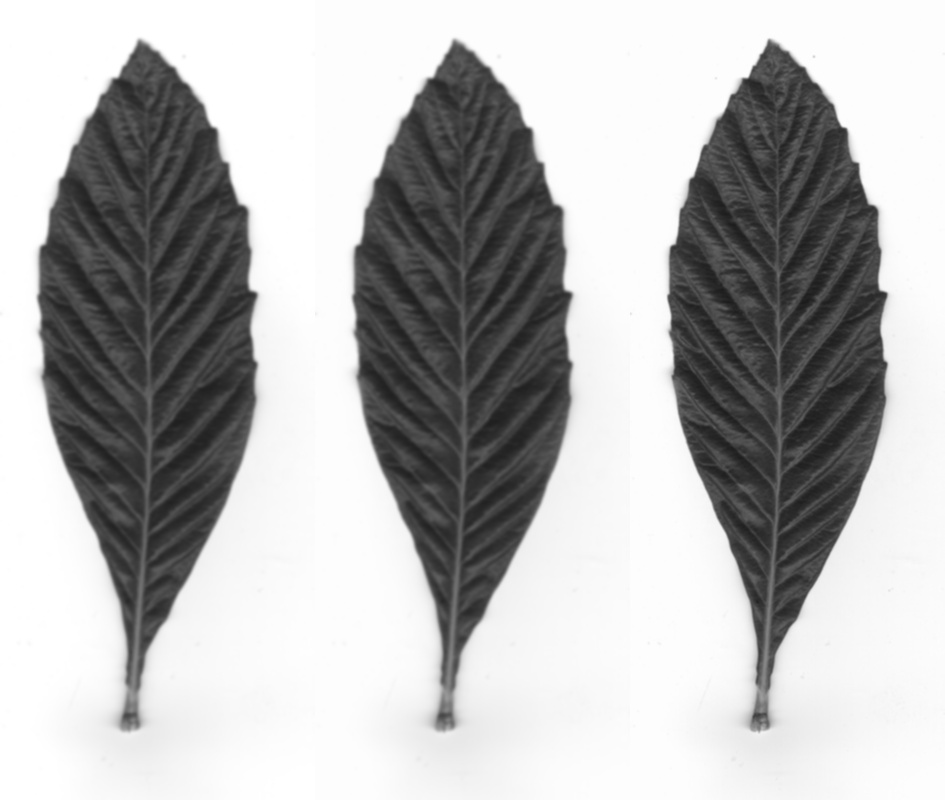
\includegraphics[scale=0.3]{blur.jpg}
    \caption{Illustration of scale factor gradient (octave 7x7;$\sigma_0$ =0; $\sigma_1$ =1.6; $\sigma_2$ =0.4) }\label{figure:Illustration of the scale factor gradient}
\end{figure}
After that, the key-points which have dimension approximately equal to $\sigma$ are detected by using the Difference of Gaussian(DoG) given by the following equation.
\begin{equation}
D(x,y,\sigma)=L(x,y,k\sigma)-L(x,y,k\sigma)
\end{equation}
Where k is the fixed parameter of the algorithm and depend to the fineness of the scale desired.
\begin{figure}[h]
    \center
    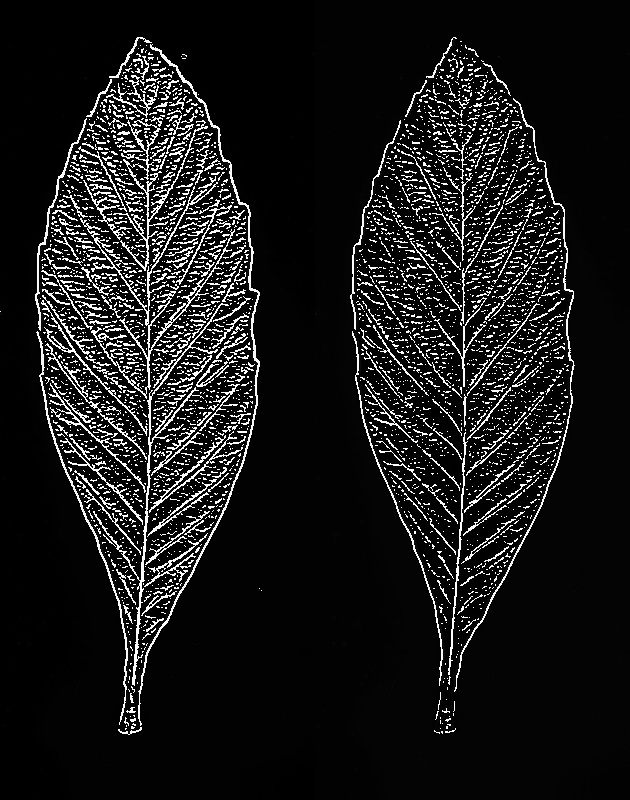
\includegraphics[scale=0.3]{DoG.jpg}
    \caption{Illustration of the DoG}\label{figure:Illustration of the DoG}
\end{figure}


\end{itemize}

\begin{itemize}
	
	\item Orientation assignment\\
	 On the base of local image gradient detections each key-point detected is assigned to one or many orientations.

  With the symmetric finite difference, the gradient and the amplitude are calculated for each position around the key-point.
The calculation of these two factors is given by the following relations:
$$m(x,y)=\sqrt{(L(x+1,y)-L(x-1,y))^2+(L(x,y+1)-L(x,y-1))^2}$$
$$\theta(x,y)=atan2(L(x,y+1)-L(x,y-1),L(x+1,y)-L(x-1,y))$$
A histogram with 36 intervals is realized on the vicinity and each interval covering an angle of 10 degrees.

 The peaks in this histogram correspond to the dominant orientations. All dominant orientations allow to have at least 80\% of the maximum value are taking in consideration and other additional key-points are detected. These new key-points detected are only different by the principal orientation.

	\item Key-point descriptor \\
An area of 16x16 pixels is taken around the key-point; subdivide in 4x4 zones of 4x4 pixels each one. A histogram including 8 intervals is calculated on each zone.

After that, the 16 histograms with 8 intervals each one, are concatenated and normalized. In object to reduce the sensibility of the descriptor to the changes of the luminosity, the values are fixed to 0.2 and the histogram is calculated again for finally give the descriptor of the key-point of 128 dimension.
\end{itemize}

\subsubsection{ SIFT test and results}

In our project we used the SIFT  of  OpenCV library in python. This function allow to detect key-points  on images and compute descriptors for each one.
The script is adapted to our program in order to calculate  descriptors in whole database of images.
Before integrating the script in the process flow, test steps were done in order to verify if the results obtained with the program are satisfied.

Tests consist to apply the sift on image according to different configurations to notice the invariance of the function to the configurations.
In a first phase, the tests were done on a basic image design on paint.
Here we have the illustration images  of the results

\begin{figure}[h]
        \centering
        \begin{subfigure}[b]{0.5\textwidth}
                \centering
                
\includegraphics[width=70mm]{test1.jpg}
        \end{subfigure}%
%        \caption{Key-points detected}
        \hfill
        \begin{subfigure}[b]{0.5\textwidth}
                \centering
                
\includegraphics[width=70mm]{lum1.jpg}
        \end{subfigure}
        \caption{Key-points detected before/after luminosity change}
        \label{fig:signature1}
\end{figure}

%\begin{figure}[!h]
%\centering     %%% not \center
%\subfigure[Key-points detected ]{
\includegraphics[width=70mm]{test1.jpg}}
%\subfigure[Key-points detected after luminosity change]{
\includegraphics[width=70mm]{lum1.jpg}}
%\caption{Illustration 1}
%\end{figure}

%\begin{figure}[!h]
   % \center
   % 
\includegraphics[scale=0.2]{scal1.jpg}
  %  \caption{Key-points detected after scale change}
   % \label{figure:Illustration }
  % \end{figure}


\begin{figure}[!h]
    \center
    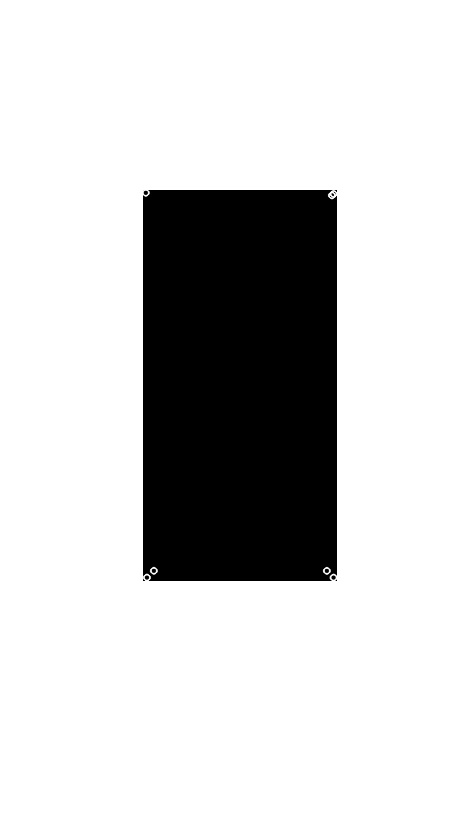
\includegraphics[scale=0.3]{rot1.jpg}
    \caption{Key-points detected after rotation}
    \label{figure:Illustration }
\end{figure}
\clearpage

After that, the test was also done on three images of the database. Three  images which look alike are taken in the database and key-points are calculated on each one.
These images are matched two by two with the key-points in order to find similarity between images.

\begin{figure}[h]
        \centering
        \begin{subfigure}[b]{0.3\textwidth}
                \centering
                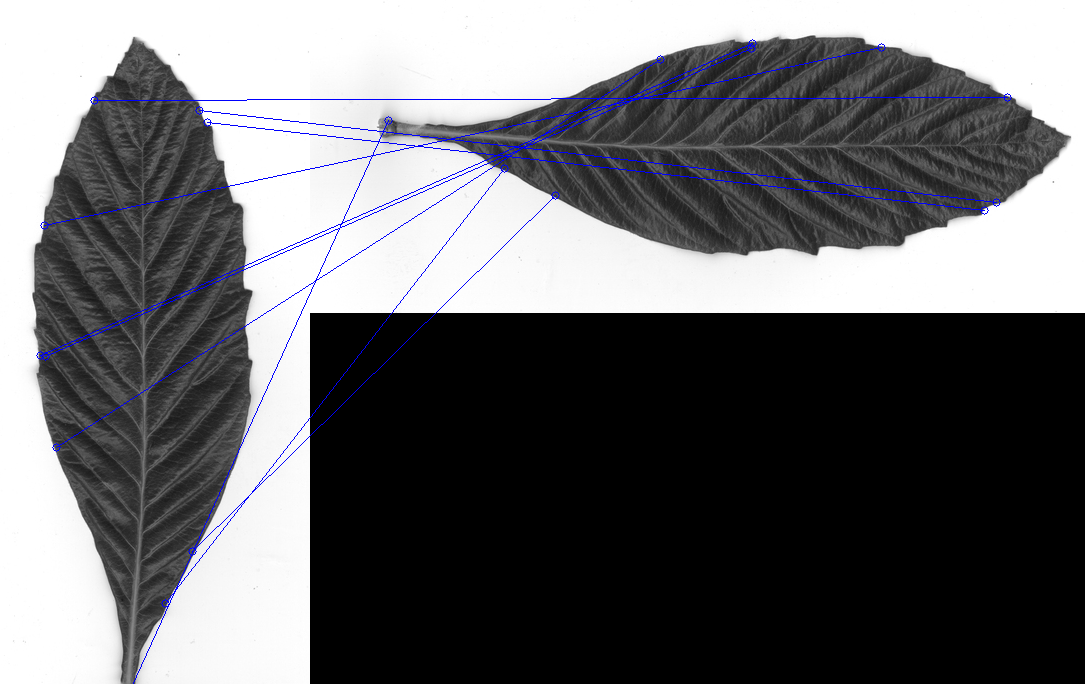
\includegraphics[width=50mm]{Capture2.png}
        \end{subfigure}%
  %      \caption{Key-points detected}
        \hfill
        \begin{subfigure}[b]{0.3\textwidth}
                \centering
                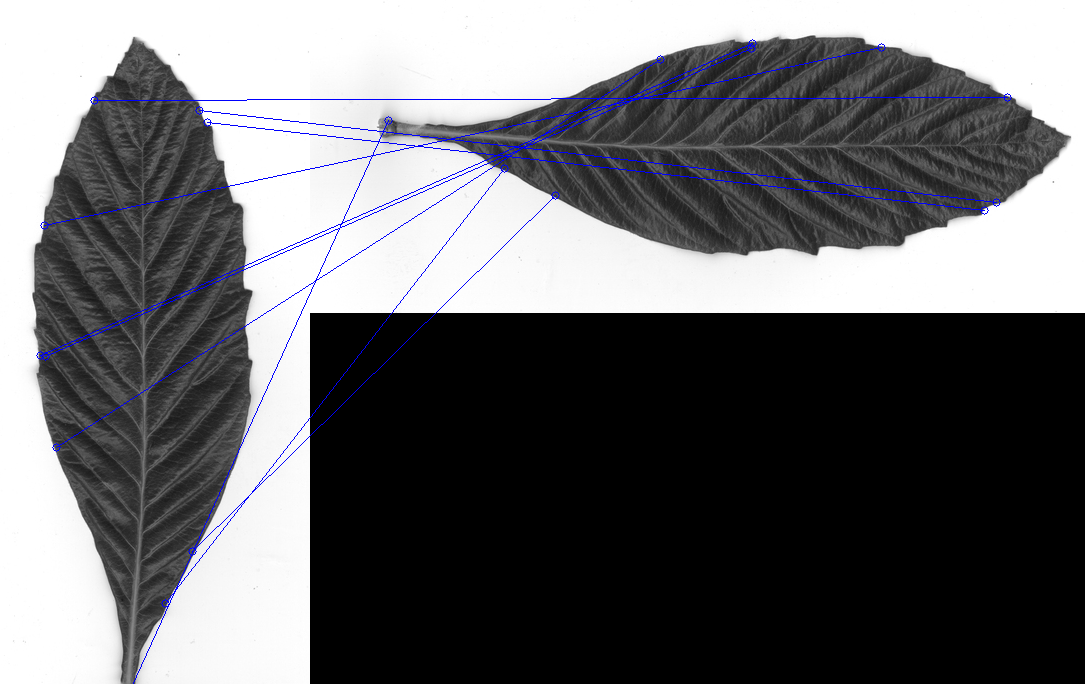
\includegraphics[width=50mm]{Capture1.png}
        \end{subfigure}
    %    \caption{Key-points detected after luminosity change
        \begin{subfigure}[b]{0.3\textwidth}
                \centering
                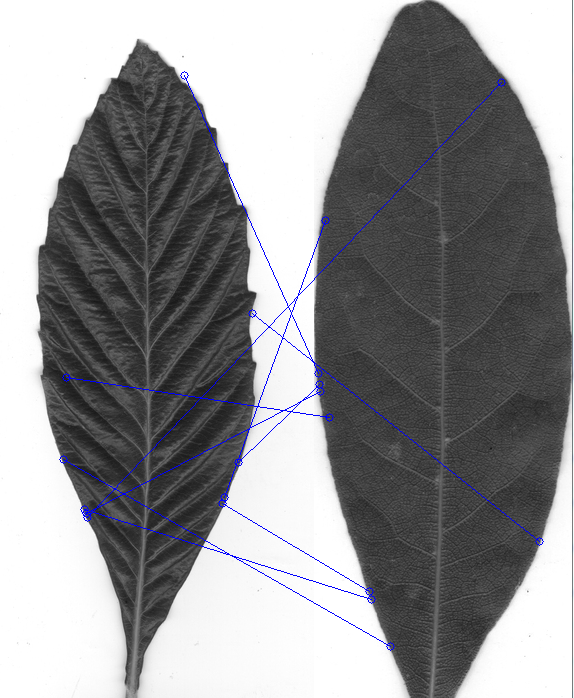
\includegraphics[width=50mm]{Capture.png}
        \end{subfigure}
        \caption{Key-points detected after luminosity change}
        \label{fig:signature1}
\end{figure}

%\begin{figure}[!h]
%\centering     %%% not \center
%\subfigure[Illustration 1 ]{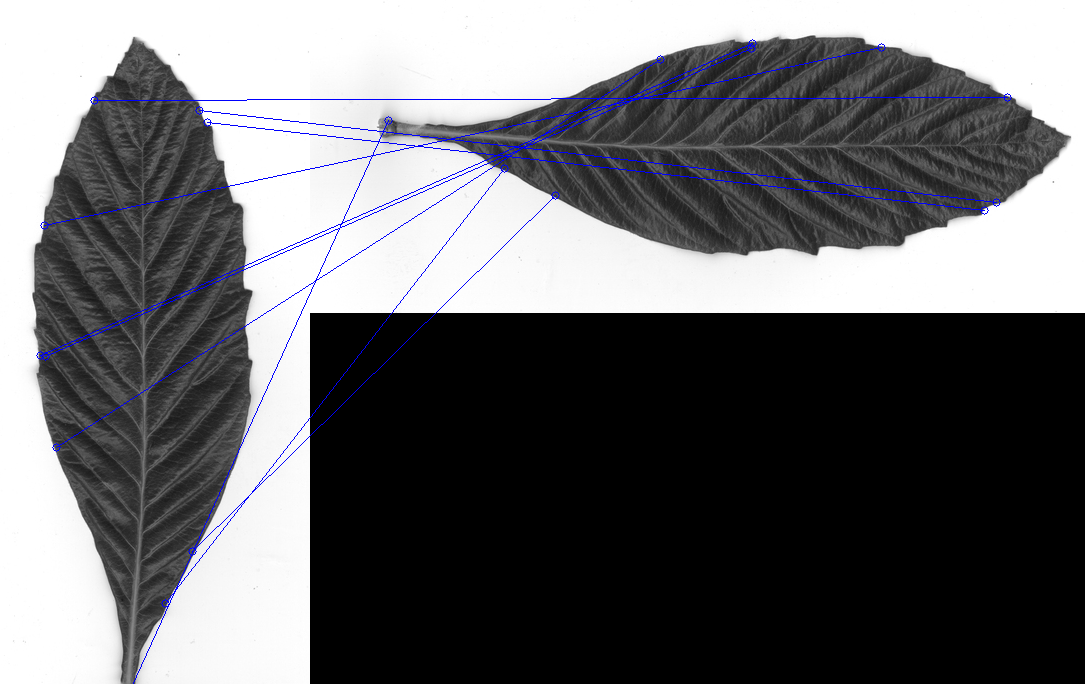
\includegraphics[width=50mm]{Capture2.png}}
%\subfigure[Illustration 3]{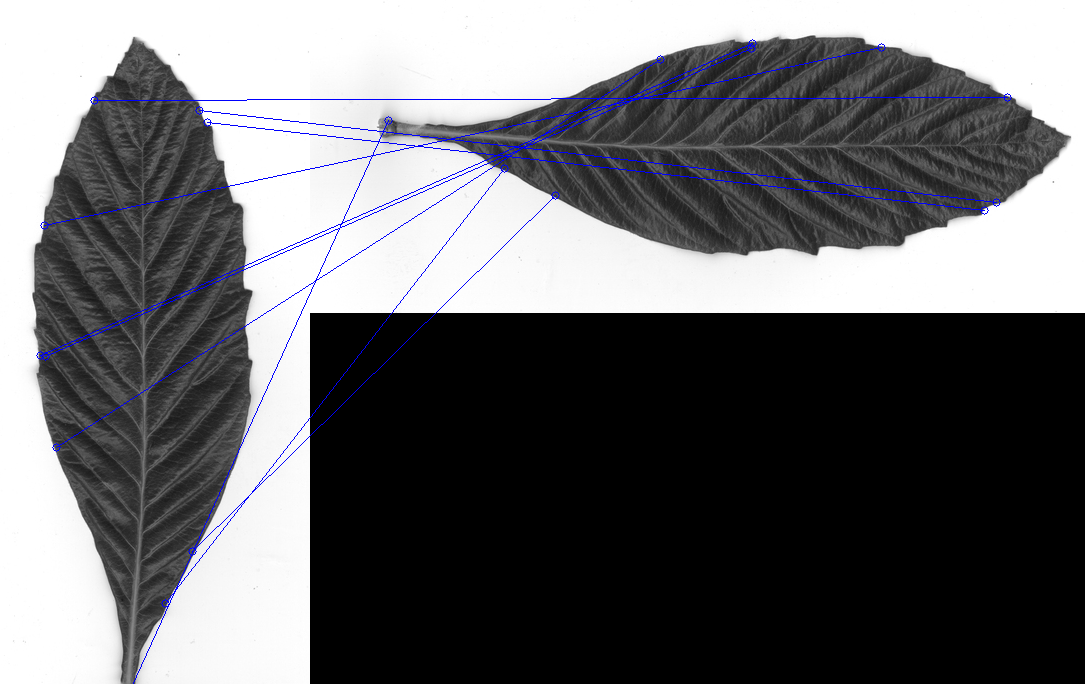
\includegraphics[width=50mm]{Capture1.png}}
%\subfigure[Illustration 3]{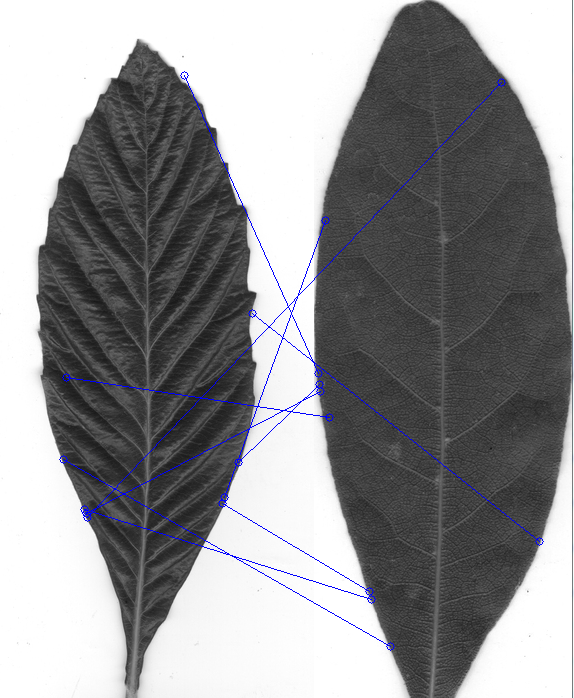
\includegraphics[width=50mm]{Capture.png}}

%\end{figure}

 According to our results obtained through the images above, we concluded that the SIFT descriptor is satisfied and it can be used to compute all descriptors in whole the database.

\subsection{ Parallelism test}

This test consist to use multiple processors to make a computation faster. It will permit multiple tasks to proceed without waiting for each other.
The algorithm consist to decompose the complete task into independent subtasks and the data flow between them and distribute the subtasks over the processors.
In python we have different possibilities to do this. The test was done by using the module multiprocessing because it was the only available in our python version.
We can see on the following images the time computation before and after using the parallelism.



\begin{figure}[h]
        \centering
        \begin{subfigure}[b]{0.5\textwidth}
                \centering
                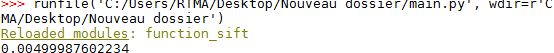
\includegraphics[width=100mm]{multi.png}
        \end{subfigure}%
  %      \caption{Key-points detected}
        \hfill
        \begin{subfigure}[b]{0.5\textwidth}
                \centering
                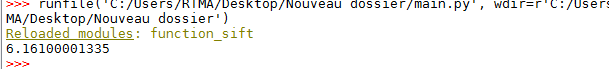
\includegraphics[width=100mm]{mult2.png}
        \end{subfigure}
        \caption{Key-points detected after luminosity change}
        \label{fig:signature1}
\end{figure}

%\begin{figure}[!h]
%\centering     %%% not \center
%\subfigure[Illustration with parallelism ]{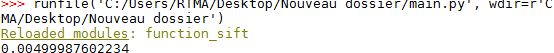
\includegraphics[width=100mm]{multi.png}}
%\subfigure[Illustration without  parallelism]{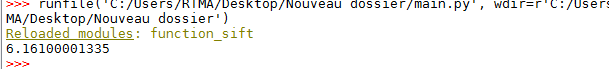
\includegraphics[width=100mm]{mult2.png}}
%\end{figure}

\newpage
\subsection{Color Constrast Occurence}

Here we will see the different steps that we have to follow to compute the C$_2$O descriptor. There will be three main steps that we will have to study, The transformation through a perceptual space, the computation of the coocurence matrix and the computation of the signature vector.

\subsubsection{Transformation through a perceptual space}

First of all, we need to pass our image in the L$^*$a$^*$b$^*$ space to get directly a representation of it in a space which split the luminance and the chromatic information.

For doing that, we first need to pass the image in the XYZ space and choose the correct standard illuminant A.
\vspace{0.5cm}
$$A=\begin{pmatrix}
	X_r&X_g&X_b\\
	Y_r&Y_g&Y_b\\
    Z_r&Z_g&Z_b
\end{pmatrix}$$


That parameter depends on the characteristics of the device used to take the picture: it represents how the device interpret real colors. In our case, there are many different devices that have been used to take the different pictures so we will have to make a choice. Some standard illuminant are defined by the illumination of the scene like D50 which corresponds to an "horizon light" contrary to D65 which correspond to a "noon light". Ideally, we will have to make the choice for each image but in front of the huge quantity of images, we had to make a choice. This choice has been to take the Adobe RGB as initial space because it's one of the most used, and to associate it with a D65 standard illuminant.

\vspace{0.5cm}
\begin{equation}
\begin{pmatrix}X\\Y\\Z\end{pmatrix}=A*\begin{pmatrix}R\\G\\B\end{pmatrix}
\end{equation}

After doing this transformation, we can easily transform our image through the L$^*$a$^*$b$^*$ space.

\vspace{0.5cm}
\begin{equation}
L^*=  \left \{
   \begin{array}{l}
      116*(\frac{Y}{Y_0})^\frac{1}{3}-16~~~~si \frac{Y}{Y_0}>0.008856\\
   903.3*(\frac{Y}{Y_0})~~~~~~~~~~si \frac{Y}{Y_0}<0.008856\\
   \end{array}
   \right .
\end{equation}
\vspace{0.5cm}
\begin{equation}
a^*=500*\begin{bmatrix}f(\frac{X}{X_0})-f(\frac{Y}{Y_0})\end{bmatrix}
\end{equation}
\vspace{0.5cm}
\begin{equation}
b^*=200*\begin{bmatrix}f(\frac{Y}{Y_0})-f(\frac{Z}{Z_0})\end{bmatrix}
\end{equation}

\subsubsection{The coocurence matrix}

To obtain the concurrence matrix, we have to calculate an image of the difference of color. For that, the program will take the difference between each point of the image and the point which is at a distance following a $\Delta$ vector from it. This calculation will has the same result if we compute the difference between the original image and a copy of it translated following $\Delta$.

\begin{figure}[h]
    \center
    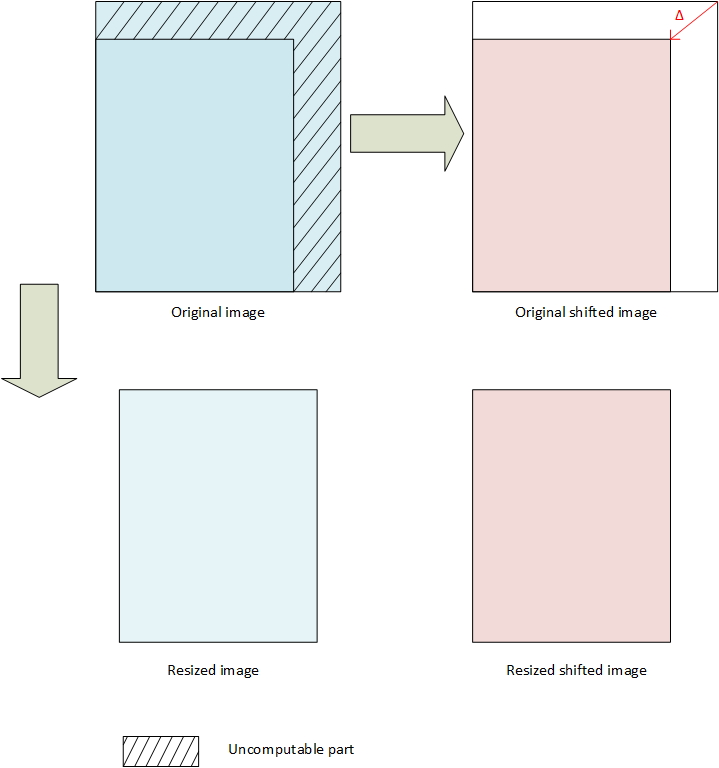
\includegraphics[scale=0.65]{ColorDiff.png}
    \caption{Color Difference illustration}\label{fig:Color Difference by image shifting illustration}
\end{figure}

To do that, the program will calculate the equivalent of the translation in horizontal and vertical pixel translation as show below .

\begin{figure}[h]
    \center
    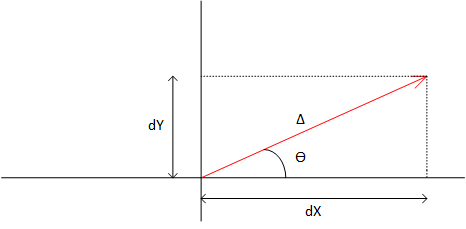
\includegraphics[scale=0.85]{illustrationVecteur.png}
    \caption{Vector to pixel distance}\label{fig:Vector to pixel distance}
\end{figure}

\begin{equation}
\begin{split}
&\sin\theta=dY/\|\Delta\| \\
&dY = \sin\theta * \|\Delta\| \\
&\cos\theta=dX/\|\Delta\| \\
&dX = \cos\theta * \|\Delta\|
\end{split}
\end{equation}

The values of $\|\Delta\|$ and $\theta$ have to being choose in the aim of get an entire number of pixel.

This computation gives us the C$_2$O matrix which corresponds to the cloud of point described in the State of art. To validate this part, we have to compare our results with theory. It's known that the L$^*$a$^*$b$^*$ space has different component :
\begin{itemize}
\item L$^*$ which is an achromatic component
\item a$^*$ which express the opposition between the red and the green
\item b$^*$ which express the opposition between the blue and the yellow
\end{itemize}


\begin{figure}[h]
    \center
    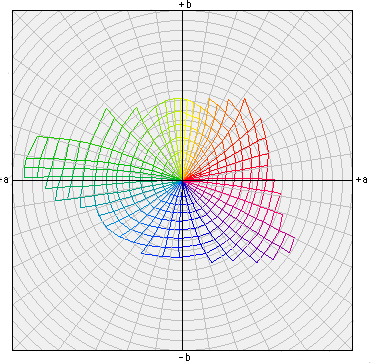
\includegraphics[scale=0.95]{BL_LAB.png}
    \caption{Lab space illustration}\label{fig:Lab space illustration}
\end{figure}
\newpage
We define two test images composed by a succession of line at different colors levels.

So if we are testing our program on images like the two one shown below which are containing the two same colors opposed on the same component of the  L$^*$a$^*$b$^*$ space, the result on the difference must show that :

\begin{itemize}
\item For the first one which is in green and red, there will be two points spaced on the a$^*$ component but at constant levels on the L$^*$ and the b$^*$ component.
\item For the second one which is in blue and yellow, there will be two points spaced on the b$^*$ component but at constant levels on the L$^*$ and the a$^*$ component.
\end{itemize}


\begin{figure}[h]
        \centering
        \begin{subfigure}[b]{0.5\textwidth}
                \centering
                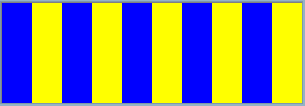
\includegraphics[height=70px]{TestIMG_BY.png}
        \end{subfigure}%
        \hfill
        \begin{subfigure}[b]{0.5\textwidth}
                \centering
                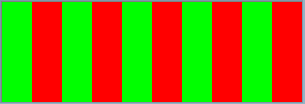
\includegraphics[height=70px]{TestIMG_RG.png}
        \end{subfigure}
        \caption{Test images}
        \label{fig:Test images}
\end{figure}

\begin{figure}[h]
        \centering
        \begin{subfigure}[b]{0.5\textwidth}
                \centering
                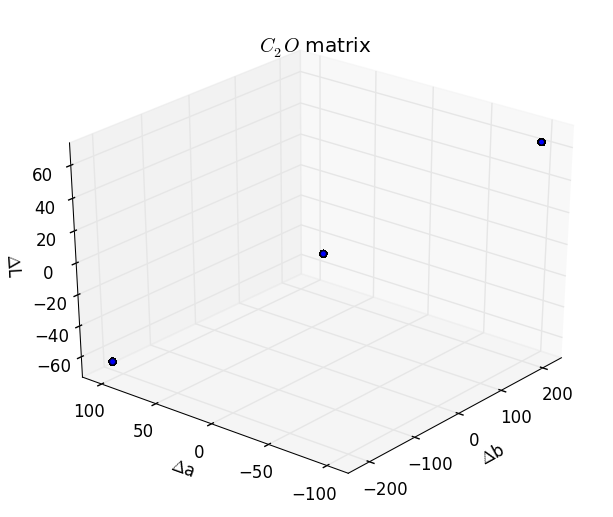
\includegraphics[height=220px]{MatriceC2O_ImgBleuJaune.png}
        \end{subfigure}%
        \hfill
        \begin{subfigure}[b]{0.5\textwidth}
                \centering
                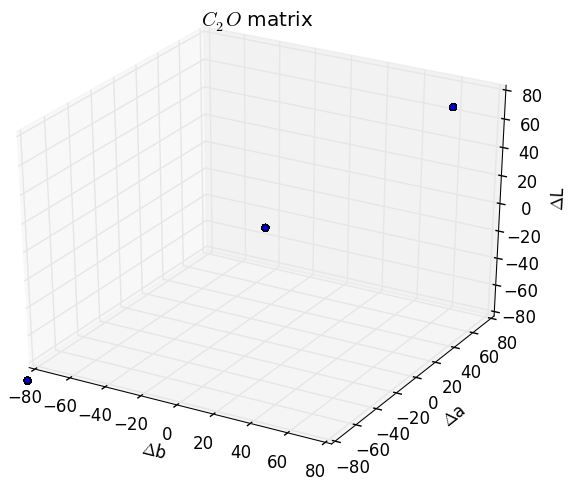
\includegraphics[height=220px]{MatriceC2O_ImgRougeVerte.png}
        \end{subfigure}
        \caption{Coorcurence matrix obtained from test images}
        \label{fig:Coorcurence matrix obtained from test images}
\end{figure}

With this step validate by the theory, we will have to test with more colors to verify that we obtain the right number of points on the coocurence matrix for the corresponding number of colors. For each test image, there will be more points as the number of colors on the image is growing because the number of difference of color will grow too.

\newpage
\subsubsection{The signature computing}

After doing that, we have to compute the spherical quantization of the probability matrix. For that, we have to transform our difference image from Cartesian coordinates to Spherical coordinates (from these one, the spherical quantization will be easier to compute). So we consider our $L^*a^*b^*$ space like a 3 dimensional repository and for each points, it's calculate E the norm of the vector formed by the distance between it and the point (0,0,0), the orientation $\alpha$ formed by the angle between the vector and the $a^*$ plan and finally the orientation $\beta$ formed by the angle between the vector and the $b^*$ plan.


\begin{figure}[h]
    \center
    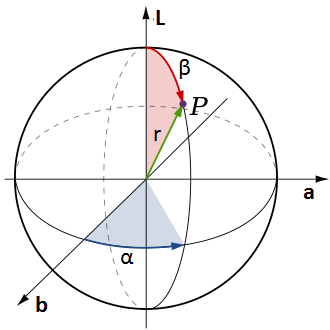
\includegraphics[scale=0.60]{Spherical_Coordinates.png}
    \caption{Spherical coordinates}\label{fig:Spherical coordinates}
\end{figure}

To calculate these coordinates, we have to use the following equations :

\begin{equation}
\begin{split}
&E = \sqrt{x^2+y^2+z^2} \\
&\alpha = \arctan(y/x) \\
&\beta = \arccos(z/r)
\end{split}
\end{equation}

So for each pixel we obtain :
\begin{itemize}
\item $\Delta$ E the color distance (approximately equivalent to the contrast)
\item $\Delta \alpha$ the orientation of the $\Lambda$ vector on the a, b plan (that give us an image of the hue)
\item $\Delta \beta$ the orientation of the $\Lambda$ vector on the L, b plan (that give us an image of the luminance)
\end{itemize}


In that way, we obtain our cloud of points in a spherical repository. Once we get it, we need to calculate our C2O signature by quantifying the cloud of point we obtain by a spherical quantization.


It's computed in three times :

There will be 4 interval of radius for the sphere :

\begin{equation}
\begin{split}
&0 \leq \Delta E < 3
\\&3 \leq \Delta E < 6
\\&6 \leq \Delta E < 9
\\&9 \leq \Delta E < infinite
\end{split}
\end{equation}


Each sphere will be split by $\alpha$ interval to concentrate the information as show below in the sectional view following the $(a^*,b^*)$ plan.
Each $\alpha$ interval will measure $\Delta\alpha=360/8$

This quantization has to be done for each value of $\beta$ interval which will measure $\Delta\beta=180/8$.

\begin{figure}[ht]
    \center
    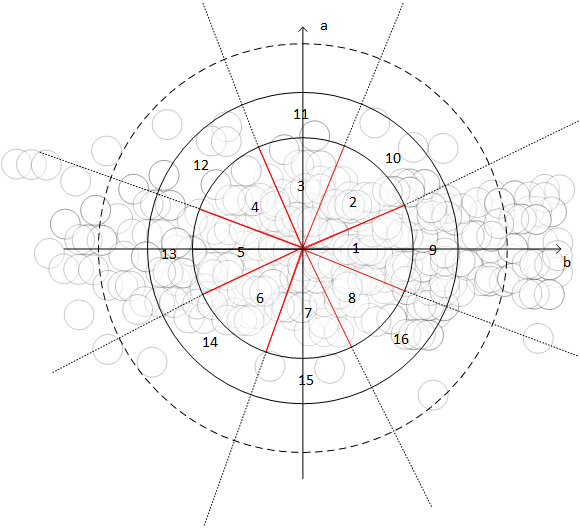
\includegraphics[scale=0.5]{QuantificationSphericToHist1.png}
    \caption{Spherical quantization following $\alpha$ and E}\label{fig:Qantification sph�rique}
\end{figure}


Once this quantization is done, the signature can be constituted by concatenate the values in a vector following a spiral for each value of $\beta$.

\begin{figure}[ht]
    \center
    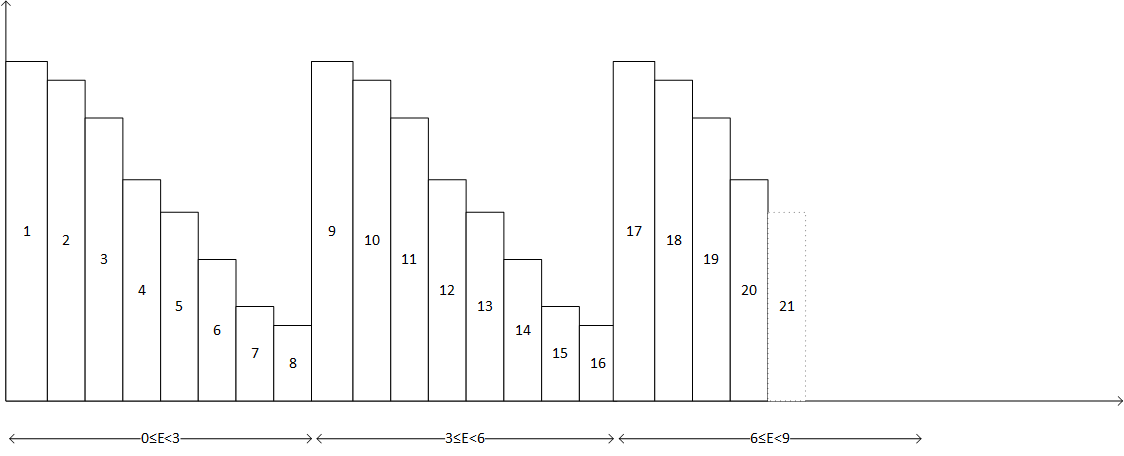
\includegraphics[scale=0.5]{QuantificationSphericToHist2.png}
    \caption{Spherical quantization following $\alpha$ and E}\label{fig:Qantification sph�rique}
\end{figure}

\newpage
The histograms obtained for each interval of $\beta$ will be concatenate to obtain the whole signature.

\begin{figure}[ht]
    \center
    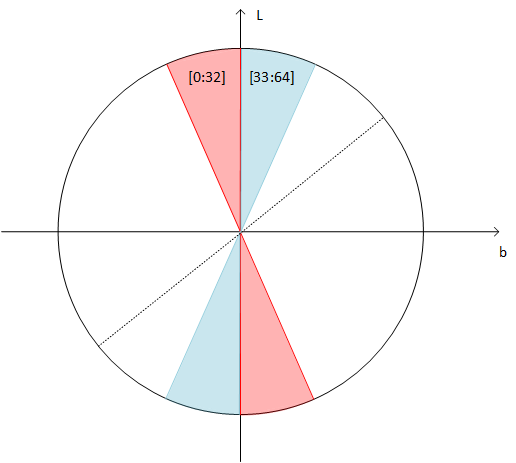
\includegraphics[scale=0.5]{QuantificationSphericToHist3.png}
    \caption{Spherical quantization following $\beta$ }\label{fig:Qantification sph�rique}
\end{figure}


\begin{figure}[ht]
    \center
    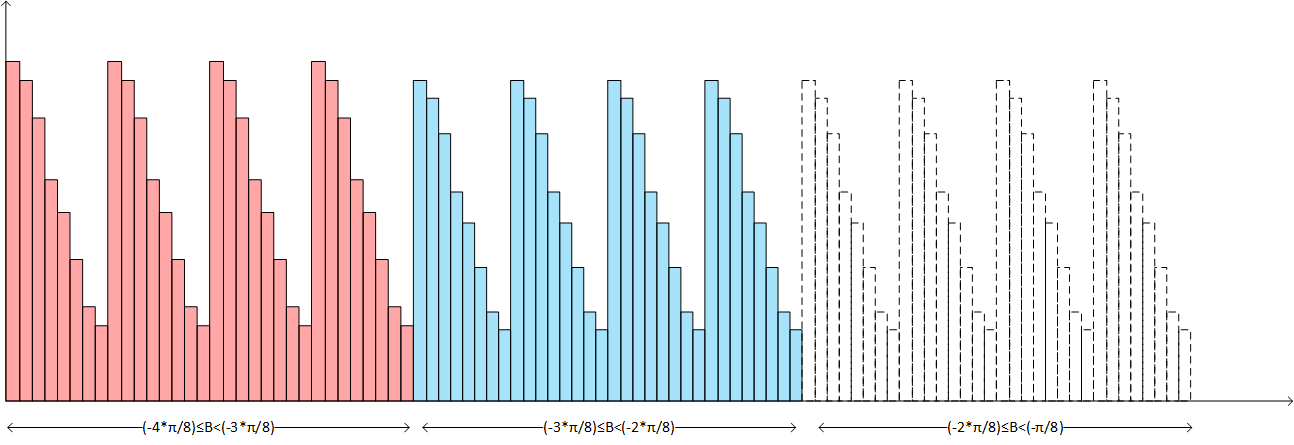
\includegraphics[scale=0.5]{QuantificationSphericToHist4.png}
    \caption{Spherical quantization following $\beta$}\label{fig:Qantification sph�rique}
\end{figure}



In this way, we obtain one unique vector of 256 values to describe the image.
\newpage
\subsubsection{Validation step}

Once these functions are computed, the most important step is to validate the good operation of all the parts. So in this part we will firstly demonstrate the functioning of the transformation through the L$^*$a$^*$b$^*$ space, an after we will talk about the spherical quantization.
The functioning of the transformation in spherical coordinates will not been covered here because of the test to validate it is just making the inverse operation and verify is we get th same data..

\paragraph{Validation of the transformation through L$^*$a$^*$b$^*$ space and color difference}
~~\\
~~\\
First of, we have to choose a reference to compare our results with. The solution choose is to compare the result of our function with those of the Bruce Lindbloom website's calculator which is a well know reference in image processing.

We has choose to work from the AdobeRGB space because it's one of the most used.
To compute correctly the L$^*$a$^*$b$^*$ space, we have to apply a $\gamma$ factor to make the operation called ��inverse companding��. This correction is made because we consider that the RGB space as it is capture by actual sensors is non linear because of the inequality of energy between low and hight luminosity levels.
The $\gamma$ inverse companding factor to apply is 2,2 and the standard illuminant is D65.
We can compare our results  with the Bruce Lindbloom website's calculator to verify that we obtain the good results.

Here we will make a first test with only 2 colors, the red and the green.
\vspace*{2mm}


\begin{equation}
\begin{split}
RGB =& [255 ,0 ,0] ~~/~~ L^* =61.4272~~  a^*=89.5619~~   b^*=75.1487
\\RGB =& [0 ,255 ,0] ~~/~~ L^* =83.3027~~  a^*=-137.9737~~   b^*=90.8299
\end{split}
\end{equation}

\vspace*{2mm}

Because of the construction of the image on which we are testing our program, there will be only to different values of color difference on each component so by calculate and compare it with the theoretical values, we could validate our color difference computation:
\vspace*{7mm}

$\Delta L_1$ = -21,8755
$\Delta a_1$ = 227,5356
$\Delta b_1$ = -15,6811

$\Delta L_2$ = 21,8755
$\Delta a_2$ = -227,5356
$\Delta b_2$ = 15,6811
\vspace*{7mm}

Here we will make a second test with Yellow and blue.
\vspace*{2mm}



\begin{equation}
\begin{split}
RGB& = [255 ,255 ,0] ~~/~~ L =97.0132~~  a=-22.5787 ~~  b=105.3055
\\RGB& = [0 ,0 ,255] ~~/~~ L =32.9786 ~~ a=80.3051 ~~  b=-109.3824
\end{split}
\end{equation}

\vspace*{2mm}
As it has been done for the first test, we will compare our result of color difference with the theoretical ones.
\vspace*{7mm}

$\Delta L_1$ = 64,0346
$\Delta a_1$ =  -102,8838
$\Delta b_1$ = 214,6879

$\Delta L_2$ = -64,0346
$\Delta a_2$ = 102,8838
$\Delta b_2$ = -214,6879
\vspace*{7mm}

These results are exactly the same obtained with our software program so we can consider that our L$^*$a$^*$b$^*$ transformation and our color difference computation are valid.


\paragraph{Validation of the spherical quantization}
~~\\
~~\\
Once we could be sure that our $C_2O$ matrix is the good one, we have to validate the operating of the spherical quantization which must extract the signature of the image from the $C_2O$ matrix.

For these tests, we will fix the number of intervals choose on each component : there are 4 intervals on $\Delta E$, 8 intervals on $\Delta \alpha$ and 8 intervals on $\Delta \beta$.
So we will obtain a signature of 256 values to describe the image. To validate our spherical quantization, we have to create a matrix in spherical coordinates in which we will fix all the values. The first test we will do is to fix our values to have all the points of our matrix in one only interval of $\alpha$. By doing that, we will be sure that the quantization is good because we will produce the values especially to be in one only interval of the final signature/histogram.

For example here we want to have all the values in the first interval of the histogram.

So the values of $\Delta E$ has to been fixed between 0 and 3, values of $\Delta \beta$ has to be between $\frac{-2 \pi }{16}$ and $\frac{2 \pi}{16}$ and the values of $\Delta \alpha$ has to be between  $\frac{-8 \pi }{16}$ and $\frac{-6 \pi }{16}$  (as show below)

\begin{figure}[H]
    \center
    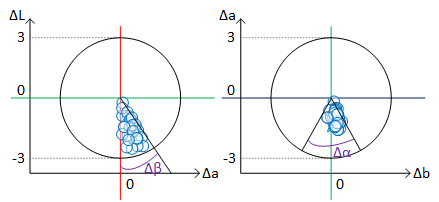
\includegraphics[scale=1]{IllustrationQuantifTheo.png}
    \caption{Quantization validation : point generation example}\label{fig:Illustration th quantif}
\end{figure}

So to do that, we generate these values by using a random function weighted by the right parameters and we obtain the following matrix�:

\begin{figure}[H]
    \center
    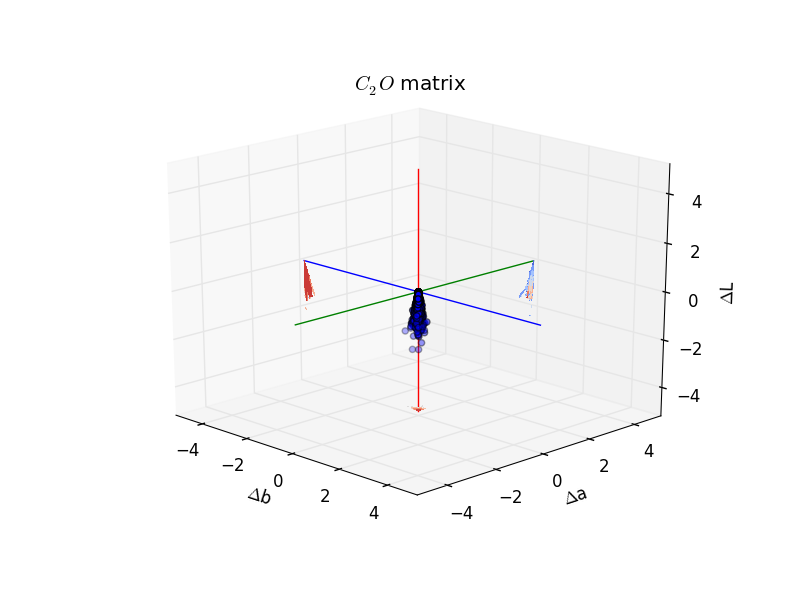
\includegraphics[scale=0.75]{QuantifInterv0.png}
    \caption{Quantization validation : point generation example}\label{fig:Illustration th quantif}
\end{figure}


Beginning with the same formulas, we are now able to write a general process to generate values in one only interval of the quantization following the calculation describe below�:
\vspace*{7mm}
\newline
$\Delta E$ = $\|(random(30,30))\|$*3 \newline
$\Delta E$ = $\Delta$ E + (3* NbInterE) \newline
$\Delta \alpha$ = $\|(random(30,30))\|$* $\frac{\pi}{8}$ \newline
$\Delta \alpha$ = $\Delta \alpha $+ $(NbInter \alpha * \frac {2* \pi}{8})$ \newline
$\Delta \beta$ =  $\|(random(30,30))\|$*$ \frac{\pi}{8}$ \newline
$\Delta \beta$ = $\Delta \beta$ � ((4-NbInter $\beta) * \frac {\pi}{8})$ \newline

For example, if we set  NbInterE to 0, $NbInter \alpha$ to 4 and  $NbInter \beta$ to 0, we must have all the 900 (30*30) values on the $4^th$ interval (8*4*0 + 8*0 + 4).

Here we can see the matrix that we obtain with these parameters�:


\begin{figure}[H]
    \center
    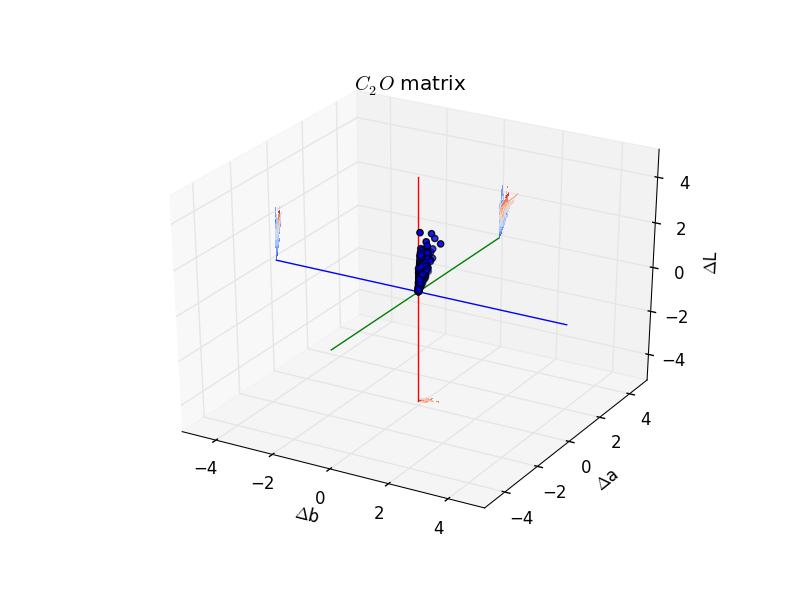
\includegraphics[scale=0.5]{MatC2OTestQuantifInterv4.png}
    \caption{C$_2$O matrix $4^{th}$ interval}\label{fig:Qantification sph�riquevalid1}
\end{figure}

So we have the following signature�:



\begin{figure}[H]
    \center
    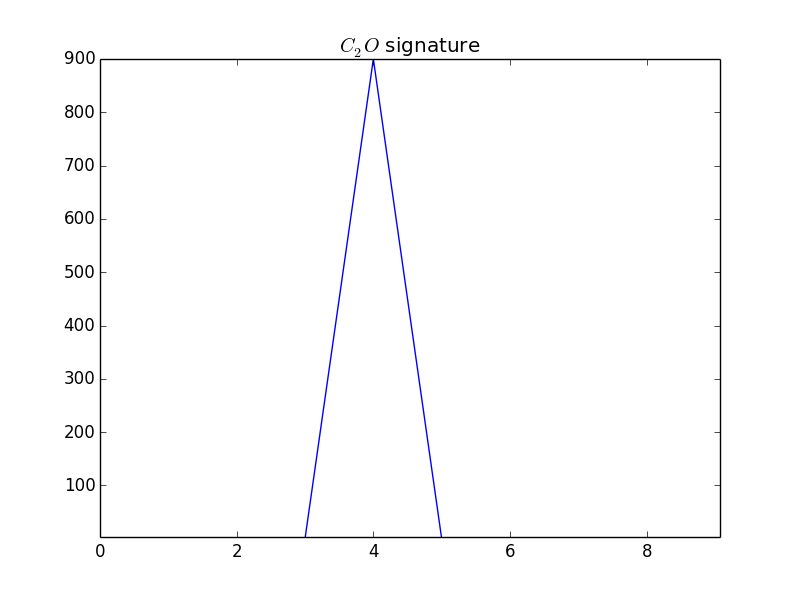
\includegraphics[scale=0.5]{SignatureTestQuantifInterv4.png}
    \caption{C$_2$O singnature $4^{th}$ interval}\label{fig:Qantification sph�riquevalid2}
\end{figure}

All the values are on the $4^{th}$ interval.

Let's test it for another interval. If we set NbInterE to 1, $NbInter \alpha$ to 3 and  $NbInter \beta$ to 1, we must have all the 900 (30*30) values on the $43^th$ interval (8*4*1 + 8*1 + 3).

The following matrix is obtained�:


\begin{figure}[H]
    \center
    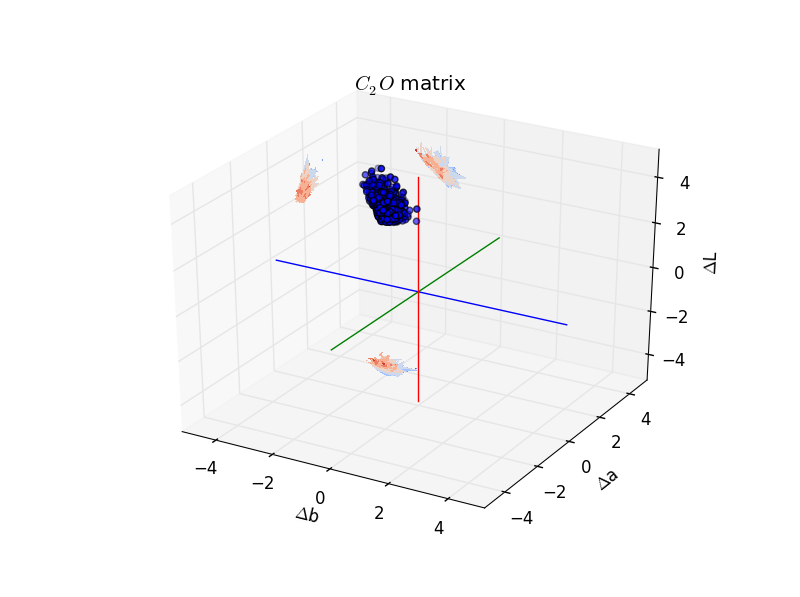
\includegraphics[scale=0.5]{MatC2OTestQuantifInterv43.png}
    \caption{C$_2$O matrix $43^{th}$ interval}\label{fig:Qantification sph�riquevalid3}
\end{figure}

So we obtain the following signature�:





\begin{figure}[H]
    \center
    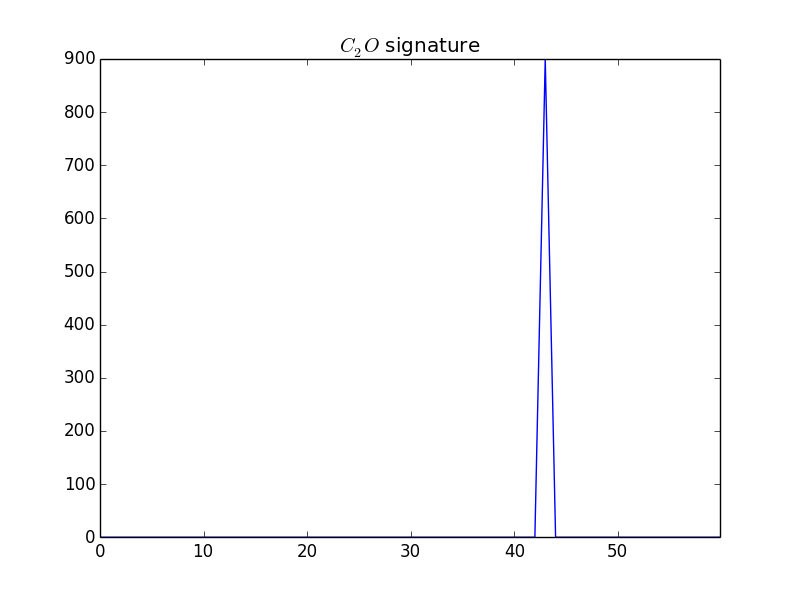
\includegraphics[scale=0.5]{SignatureTestQuantifInterv43.png}
    \caption{C$_2$O signature $43^{th}$ interval}\label{fig:Qantification sph�riquevalid4}
\end{figure}

All the values are on the $43^{th}$ interval.

Considering these results, we can validate operation of our spherical quantization.

\newpage
\subsection{Metadata}

    The image database come with xml files containing associated with every pictures respecting the format below :
\begin{figure}[H]
  \centering

  \includegraphics[width=8cm]{captureXML.png}\\
  \caption{\small \it {metadata of the picture number 2}}
\end{figure}

Among those, only the following can be useful :
\begin{itemize}

\item ObservationId: the plant observation ID from which several pictures can be associated, represents a unique environment (same plant, same day, same author);
    \begin{figure}[H]
      \centering
      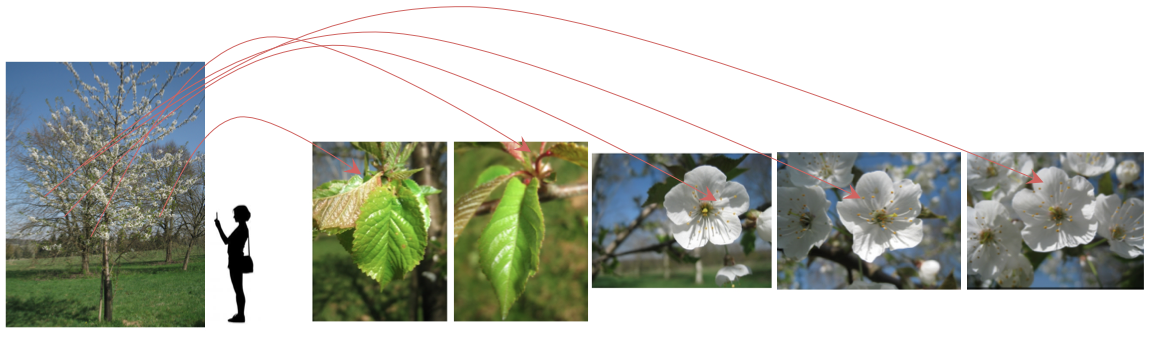
\includegraphics[width=10cm]{OnePrunus.png}
      \caption{\small\it{One observation of one individual-plant observed the same day by a same author involving several pictures with the same Observation ID}}
    \end{figure}

\item content: part of the plant represented in the picture : "Leaf", "Flower", "Fruit", "Stem", "Entire", "Branch", can be used to in the prediction process;
\item ClassId: the class number ID that must be used as ground-truth. It is a numerical taxonomical number used by Tela Botanica, unique to each species;
\item Species: the species names (containing 3 parts: the Genus name, the Species name, the author(s) who discovered or revised the name of the species);
\item Family: the name of the Family, two levels above the Species in the taxonomical hierarchy used by Tela Botanica;
\item author: name of the author of the picture, will be of use to balance the metrics ;
\end{itemize}

\subsubsection{metadata retrievers}
    Every picture of the dataset is bundled with a XML file providing related data.
    Retrieving relevant data from those files was necessary in order to associate the results of the descriptors with what they represent. Metadata can also be used to limit the database to a un unique family, to certain species or to a specified content(branch, fruit, etc).

    For this purpose we created a function which look into those files to return the observationId, classId, author, etc.

\subsubsection{relevant metadata storing}
    At first we expected to recreate a single XML file containing only the relevant metadata so that we don't have to rescan the data bank each time we need something.
    But the XML format didn't turn to be very practical to use since when reading the files it was not possible to retrieve the parent from the nodes. And without using a tree structure, the XML format loses some of its appeal.

    We switched for a simple text file providing with each lines the observationID, the ClassID, the file related and the author.


\subsubsection{XML handling}

 For some reasons, at the beginning we had decided to use XML files files to store the keypoints and their coordinates. The idea was to have something like that :

 \lstset{language=XML}

 \begin{lstlisting}
<?xml version="1.0" encoding="utf-8"?\>
 <keypoints>
    <kp1>
        <x></x>
        <y></y>
        <xs:descriptor></xs:descriptor>
    </kp1></kp2>
        <x></x>
        <y></y>
        <descriptor>
        </descriptor>
    </kp2>
 </keypoints>
\end{lstlisting}




The idea was discarded later as it turned out there was no benefit with this and a simple text file containing at each line
\quote{x y descriptor} was more than enough and easier to do.
\newpage
\subsection{Quantization}

The Quantization is the step we will use for determine which images correspond to which species. For that we will use the bag of words in a first place to simplify the signature of whole images. And after use the K-nn method for the classification.

\subsubsection{Bag of words}

In the bag of words method we found two different step, the calculation of K-means and the design of a signature for the images.

\paragraph{K-means}
~~\\
~~\\
The K-means is a simply method which consist to reduce the number of points or vectors in our case. The first step is to determinate randomly k centroid vectors, after with an Euclidean distance \eqref{euclid} we attribute the descriptors to whole images to the nearest centroid vectors.

\begin{equation}
\sum_{k=0}^{centroid}\sum_{i=0}^{desc}\parallel x_k - u_i \parallel ^2
\label{euclid}
\end{equation}

The last stage is an update step, for each centroid vectors we calculate the means of whole the descriptors associate to, so we obtain a new centroid vectors. And we applicate this algorithm for x iteration choose by the user.

For an application on a cloud of points we obtain this kind of result:


\paragraph{Signature}
~~\\
~~\\
The creation of the signature is the last step of the bag of words method, they consist to assign to each images a signature in function of the number of word in the image. The graphic representation of this signature is a histogram:

\begin{figure}[H]
        \centering
        \begin{subfigure}[b]{0.5\textwidth}
                \centering
                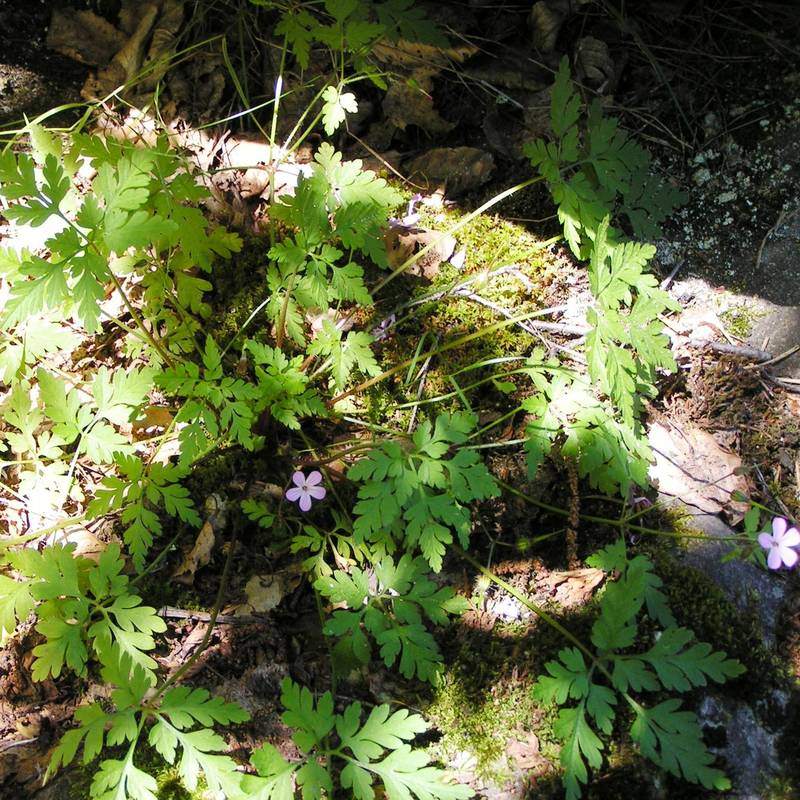
\includegraphics[height=180px]{128.jpg}
        \end{subfigure}%
        \hfill
        \begin{subfigure}[b]{0.5\textwidth}
                \centering
                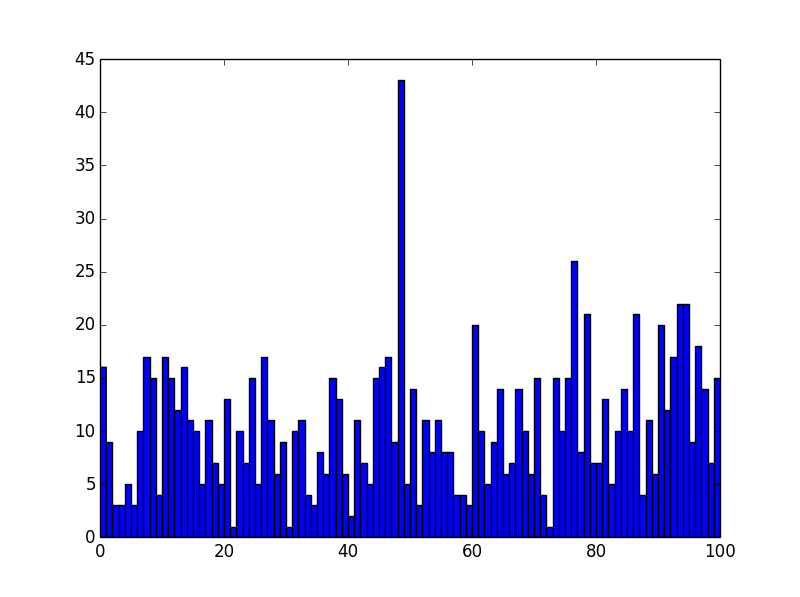
\includegraphics[height=180px]{128_sig.png}
        \end{subfigure}
        \caption{Signature de l'image 128}
        \label{fig:signature1}
\end{figure}
\begin{figure}[H]
        \centering
        \begin{subfigure}[b]{0.5\textwidth}
                \centering
                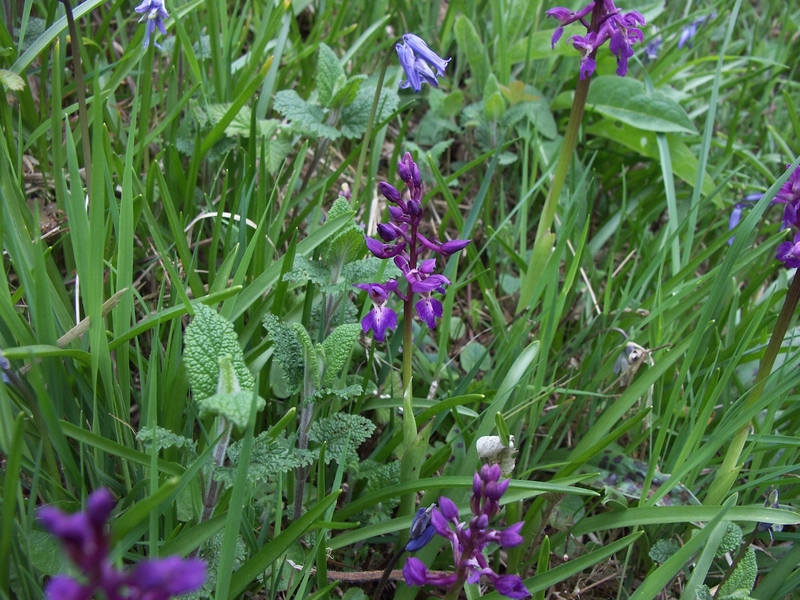
\includegraphics[height=180px]{132.jpg}
        \end{subfigure}%
        \hfill
        \begin{subfigure}[b]{0.5\textwidth}
                \centering
                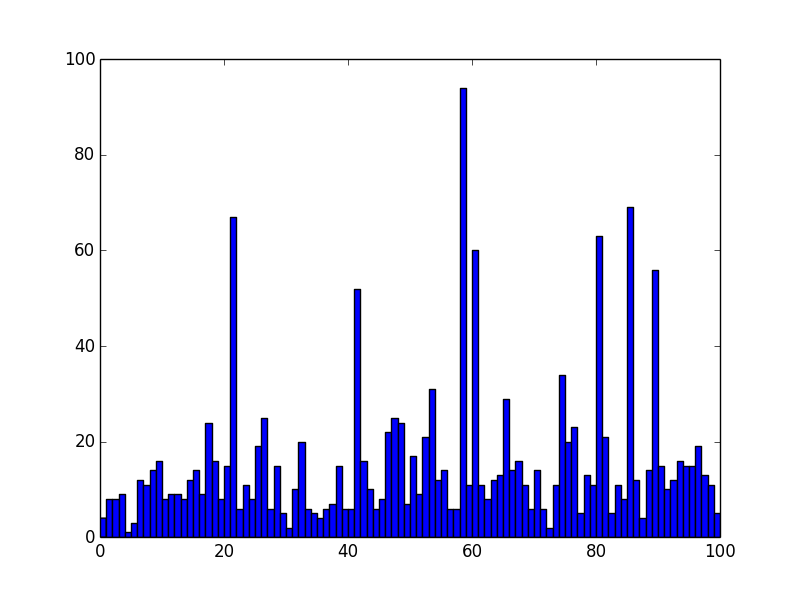
\includegraphics[height=180px]{132_sig.png}
        \end{subfigure}
        \caption{Signature de l'image 132}
        \label{fig:signature1}
\end{figure}

\subsubsection{K-nn}

\paragraph{The K-nn method}
~~\\
~~\\
The K-nn method is one of the most simple technique in the classification field. This method consist in associating the data to classify with the class that correspond the best to it.
It is a supervised learning method : it means that the k-nn has to have a dictionary which contains all the training data sorted by class. To classify a new data, the k-nn calculates the distance between each training data and the new data. After doing that, it will simply takes the 'k' smallest ones, and determine in which class t have to attribute the new data by taking the one which is the most occurrent in the 'k' smallest distances.

For our project, the data to classify are images and the classification is made by the signature vector extracted by the K-means method. The principle is exactly the but the distances are calculated on the signature vector.
We had choose two possibilities for the distance calculation : the Euclidian distance and the $\chi^2$ distance which are described below.
\begin{itemize}
\item Euclidian distance
\vspace{0.5cm}
\begin{equation}
D_{Euc}(v_1,v_2) = \sum{(v_1(i)-v_2(i))^2}
\end{equation}

\item $\chi^2$ distance
\vspace{0.5cm}
\begin{equation}
D_{\chi^2}(v_1,v_2) =  \sum{\frac{(v_1(i)-v_2(i))^2}{(v_1(i)+v_2(i))^2}}
\end{equation}

\end{itemize}

The choice of the type of distance calculation depends on the type of descriptor chosen for the classification. For SIFT descriptor,the Euclidian distance is appropriate but each descriptor must have one distance which work better than others.
That's why the $\chi^2$ distance has been integrate in the program.

\paragraph{Validation step}
~~\\
~~\\
To validate this classification method, the most simple way is to test it on artificial signatures with different constant values.
The test to validate is to take as our initial dictionary 7 vectors which we consider to be in 2 different classes. These vectors are full of constant values, they are shown as lines blow :

\begin{figure}[h]
    \center
    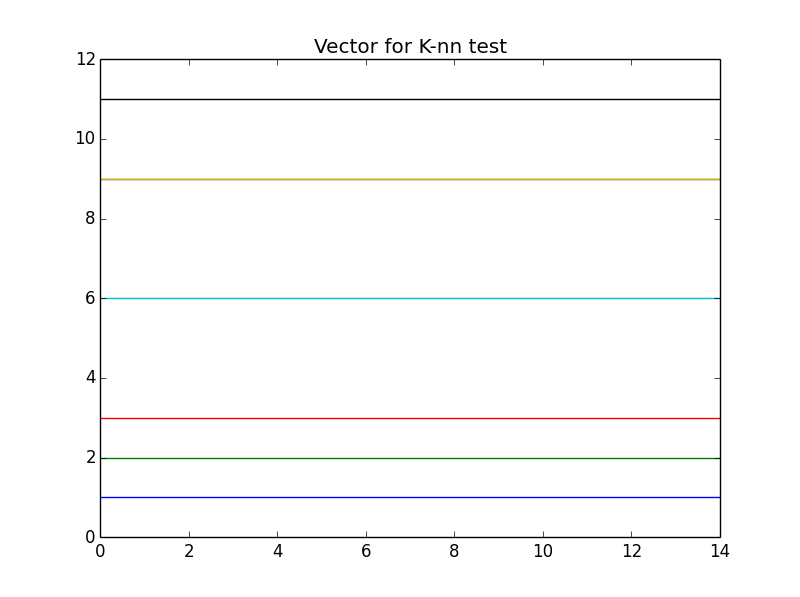
\includegraphics[scale=0.65]{knnTestVec.png}
    \caption{Dictionary of vector for k-nn tests}\label{fig:Color Difference by image shifting illustration}
\end{figure}

The lowest one (from 0 to 3) are attributed to the first class and the others are attributed to the second one.
After that, we simply have to test to classify a signature which is constructed on the same model. When the signature vector is closer of 3 than of 6, he has to be attributed to the first class, and to the second when he is closer of 6.

The result obtained by our K-nn function is the same that the one we expected so we can say that the functioning of it is valid.


\newpage
\subsection{Metrics}

    The first thing to do is to create a file with the results of the run and the related information.

    The official run files to be submitted to the challenge have to follow a specified format :

    \begin{quote}
        ObservationId;ClassId;rank;score
    \end{quote}

    The ObservationID was explained previously and is here to represent the environment of the picture (being unique to a set of an author, a place, a date and a plant)
    The ClassID represents the plant supposed to be on the picture by the classification
    The rank represents the occurrence of the same ObservationID in order to
    The score is a confidence score of a prediction item (the lower the score the lower the confidence).

    Another optional run file, detailing species prediction at image level) could be submitted as below :

    \begin{quote}
      test\_image\_name.jpg;ClassId;rank;score
    \end{quote}



    Since we didn't produce any run we left the score aside.

    Once those files produced we can now measure the performance of the run.

    The first thing to do is to check if the predicted plants are right and then to retrieve only the correct guesses.

    The CLEF challenge offers two metrics :

    The primary metric used to evaluate the submitted runs will be a score related to the rank of the correct species in the list of the retrieved species.
    Each plant observation test will be attributed with a score between 0 and 1 : of 1 if the first returned species is correct and will decrease quickly while the rank of the correct species increases. An average score will then be computed on all test individual plant. A simple mean on all observation test would however introduce some bias. Indeed since the PlantCLEF dataset was built in a collaborative manner, some contributors have provided much more observations pictures than the others. O in order to evaluate the ability of a system to provide correct answers to all users, the mean of the average classification rate per author is used.


    1st metric (score observation):


      $S1=\frac{1}{U}\sum_{u=1}^{U}\frac{1}{P_{u}} \sum_{p=1}^{P_u}S_{u,p}$


    \begin{quote}
        \begin{description}
            \item[U :] number of photography authors with at least one image in the test data
            \item[P$_u$ :] number of individual plants observed by the u-th user
            \item[S$_{u,p}$ :] score between 1 and 0 equals to the inverse of the rank of the correct species (for the p-th plant observed by the u-th user)
        \end{description}
    \end{quote}

The secondary metric is used with the optional run file providing species determination at the image level. Same as above, in order to avoid the bias brought with the fact that some authors provided many pictures of the same plant, the average classification rate on each plant is used.




    2nd metric (score image):


      $S2=\frac{1}{U}\sum_{u=1}^{U}\frac{1}{P_{u}} \sum_{p=1}^{P_u}\frac{1}{N_{u,p}} \sum_{n=1}^{N_{n,p}}S_{u,p,n}$


\begin{quote}
        \begin{description}
            \item[U :] number of photography authors with at least one image in the test data
            \item[P$_u$ :] number of individual plants observed by the u-th user
            \item[N$_{u,p}$ :] number of individual plants observed by the u-th user
            \item[S$_{u,p,n}$ :] score between 1 and 0 equals to the inverse of the rank of the correct species (for the n-th picture taken from the p-th plant observed by the u-th user)
        \end{description}
    \end{quote}

\subsubsection{score results}
We didn't manage to evaluate our own scores but the results from the challenge are available to check with.

\begin{figure}
  \centering
  \includegraphics[width=10cm]{results-image.png}
  \caption{Score 2014}
\end{figure}



\subsubsection{checking the predictions}
Once the predictions are done we still have to check whether they are correct or not. To handle this task we created a function storing the metadata and checking if the output classID linked with the filenames.

The right answers are then stored separately in order to be used for the metrics.



\newpage
\subsection{Results}

In this part, we will present the result we obtained in this project. We divide this section in two subsections, the first is the procedure we use for testing our descriptors. And the second is the presentation of the results and the comparison of the two descriptors.

\subsubsection{Procedure}

\paragraph{For one image}
~~\\
~~\\
In a first place, we use the result of the K-means for classify one image taking training database as reference:

\begin{figure}[h]
    \center
    \includegraphics[scale=0.95]{proced.png}
    \caption{Classification for one picture}\label{fig:proced1}
\end{figure}

For the SIFT descriptor we will compare the Euclidean distance \eqref{Disteuclid} and the $\chi^2$ distance \eqref{Distki}. The comparison of these distances in the C$_2$O algorithm is made in the K-means algorithm.

After the distance calculation we use the K-nn algorithm to find the species of the picture.

\begin{equation}
T_{E}(H^1,H^2) = \sqrt{\sum_{i=1}^{n} (h_{i}^{1} - h_{i}^{2})^2}
\label{Disteuclid}
\end{equation}

\begin{equation}
T_{\chi^2}(H^1,H^2) = \sum_{i=1}^{n} \frac{(h_{i}^{1} - h_{i}^{2})^2}{(h_{i}^{1} + h_{i}^{2})^2}
\label{Distki}
\end{equation}

\vspace{2cm}

\paragraph{For a database}
~~\\
~~\\
For a database we use the same method that we use for one image. For the treatment of a database we can use two different method:

\begin{itemize}
\item cross-classification

\begin{figure}[h]
    \begin{minipage}{0.50\linewidth}
        \includegraphics[scale=0.7]{proced2.png}
        \caption{Classification for a database}\label{fig:proced2}
    \end{minipage}\hfill
    \begin{minipage}{0.55\linewidth}
        The difference is that we will take 80\% of the images as a training base, and 20\% as test. The 20\% are choose randomly, but to have a means of the whole database result, we will iterate this process, and the signature of the images choose at the previous iteration can not be in the 20\% of test.
    \end{minipage}
\end{figure}

\newpage
\item let

\begin{figure}[h]
    \begin{minipage}{0.50\linewidth}
        \includegraphics[scale=0.7]{proced3.png}
        \caption{Classification for a database}\label{fig:proced3}
    \end{minipage}\hfill
    \begin{minipage}{0.55\linewidth}
        In this second method, we choose the same training base (70\% of the database), and the same test base (30\% of the database). This method allows us to see the difference between two different distance, or between the SIFT and the C$_2$O.
    \end{minipage}
\end{figure}

\end{itemize}

In scope of respecting our project schedule we have to present results so we will use the second method to have results to compare.

\subsubsection{Analysis of result}


\newpage
\section{User manual}

\newpage
\section{Project management}

\newpage
\section{Conclusion}



%-------------------Bibliography----------------------------------
\bibliographystyle{plain}
\bibliography{User_requirements}
% ----------------------------------------------------------------


%-----------------------------------------------------------------
%-------------------ANNEXES---------------------------------------
\newpage
\appendix

% ----------------------------------------------------------------
\end{document} 